%%%%
\section{África Subsariana}

A África Subsariana (SSA) é atualmente região no mundo que tem a maior taxa de 
transição da população rural - ainda predominante - para cidade 
\citep{MONTGOMERY2008}.

Pesquisas recentes tem avaliado a poluição do ar em favelas 
(regiões periféricas) \citep{SCLAR2005} e \citep{RILEY2007}. 

Mesmo assim, as cidades da \textit{SSA} ainda não possuem sistemas de 
monitoramento sistemático de poluição do ar e suas implicações na saúde 
\citep{EZZATI2004}. 
Além disso há poucas pesquisas acadêmicas dos níveis de poluição do ar nos 
países da \textit{SSA}.

Diferente dos países industrializado, onde as principais fontes de poluição 
são os setores da industria e do transporte, os países da \textit{SSA} tem como 
principal fonte poluidora a queima de biomassa, sendo comum o uso no cozimento 
de alimentos, tanto em regiões urbanas quanto rurais \citep{SMITH2004}.

Diferente das cidade dos países desenvolvidos, que tem como principais 
fontes de poluição a industria e o transporte, nas cidade da SSA as fontes 
tem outro perfil, pois na SSA:
  \begin{itemize}
    \item população predominantemente rural
    \item muitas vias não pavimentadas
    \item maior taxa de crescimento populacional urbano do mundo
    \item não possuem sistemas de monitoramento sistemático de Poluição do Ar
    \item é comum o uso da queima de biomassa para o cozimento de alimentos  
          (comercial e doméstico), tanto em regiões urbanas quanto rurais.
  \end{itemize}

%%%%
\section{Acra}

Acra é a capital  de Gana e está localizada no Golfo Guiné. Ela tem uma área 
total de mais de 2500 $km^2$ com elevação que varia de 0 até 100 pés do nível 
do mar. 
A população da região metropolitana de Acra estava em torno de 2 milhões em 2005, 
último censo disponível.
%TODO: (citar censo). 

%%%%
\section{Nima}

\begin{figure}[H]
  \caption{Fotos do bairro de Nima}
  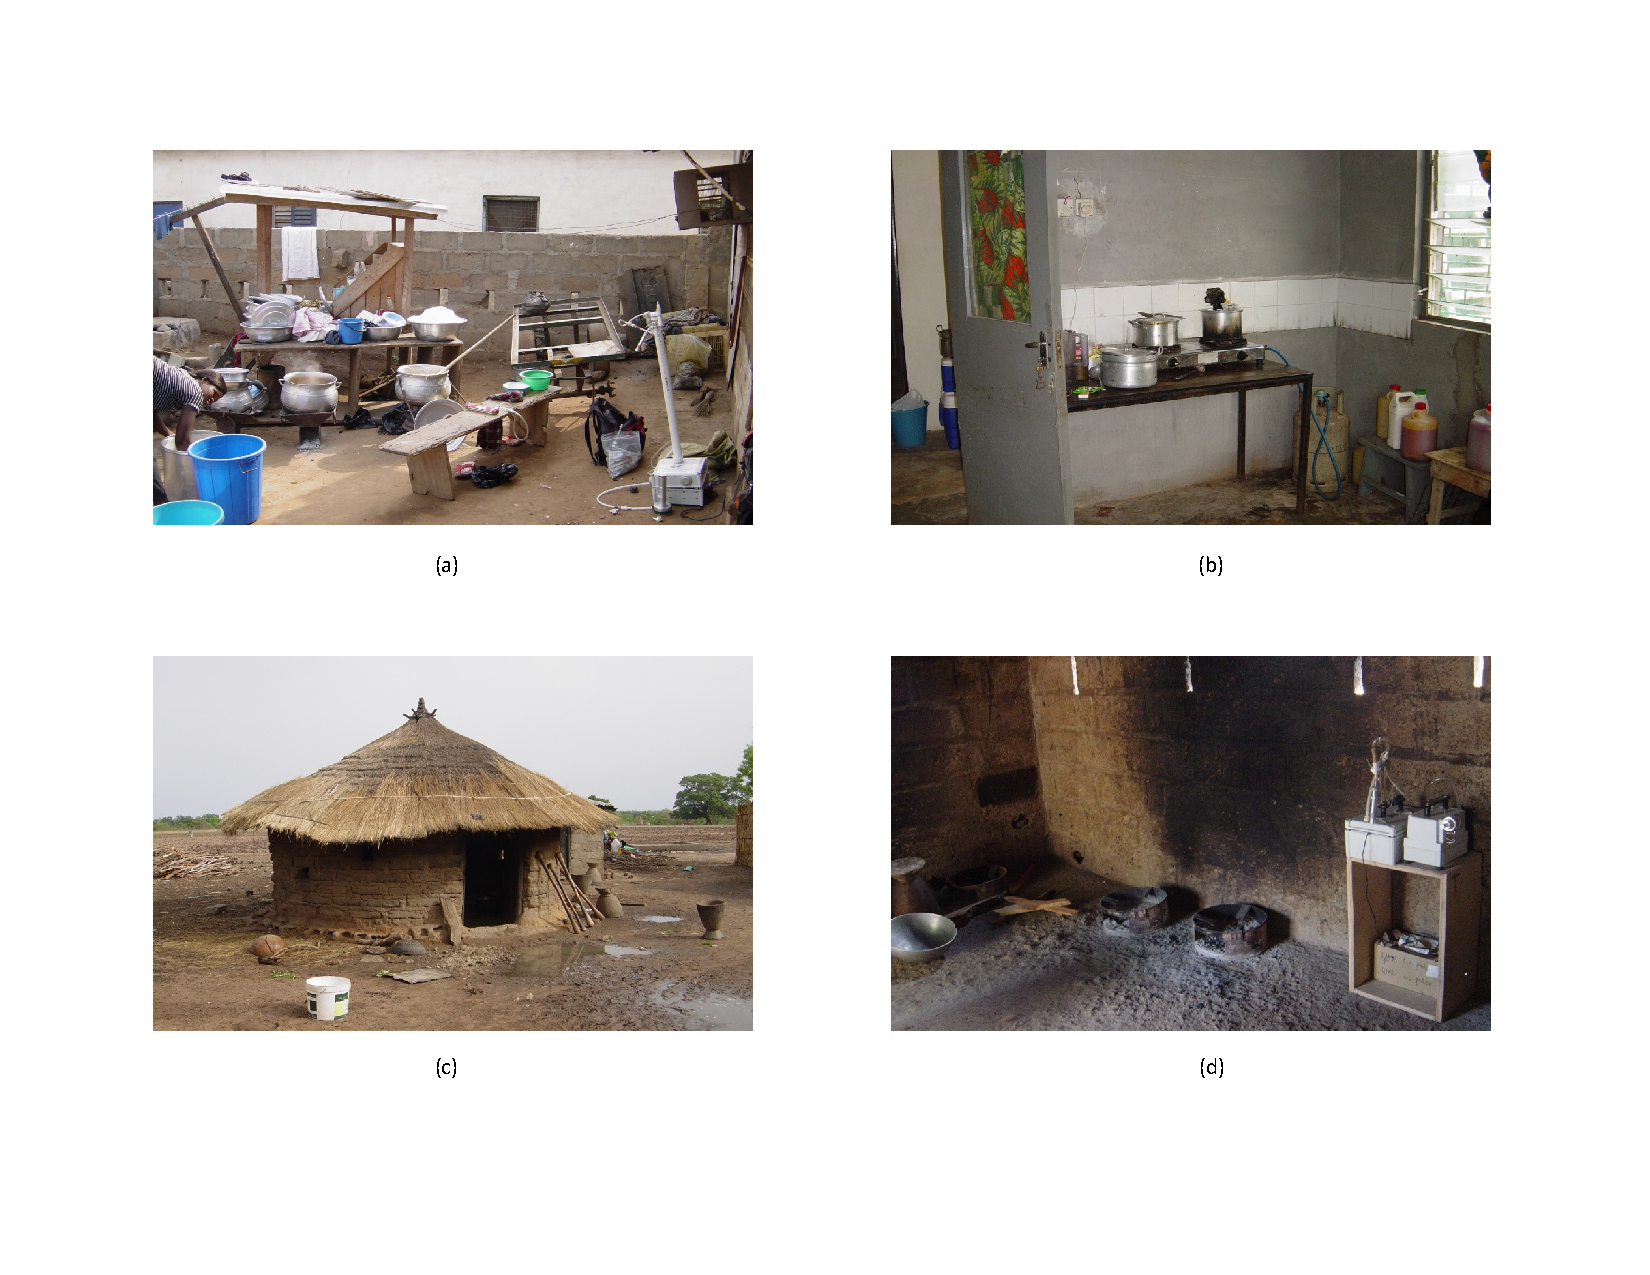
\includegraphics[scale=0.35]{../inputs/images/zheng/nima.pdf}
\end{figure}

%%%%
\section{Projeto Internacional}

Coordenado por pesquisadores da \textit{Harvard School of Public Healt} nos 
Estados Unidos, com participação da Universidade de Ghana.

O grupo de Harvard \citep{ARKU2008} conduziu um levantamento nos níveis de 
poluição, bem como da distribuição espacial e temporal de alguns poluentes 
em duas regiões periféricas de Acra \citep{DIONISIO2010}:

\begin{itemize}
  \item Jamestown/Ushertown: região entre a Costa e o centro comercial local.
  \item Nima: Centro comercial de Acra, cercada com Rodovia.
\end{itemize} 

Nos dois bairros há poucas ruas pavimentadas, com exceção das principais 
avenidas. 
